\documentclass[calcdimensions,landscape,letterpaper]{powersem}
\usepackage{color}
\usepackage[pdftex]{thumbpdf} % For thumbnails
\usepackage[pdftex]{hyperref} % For links.
\usepackage[display,coloremph,whitebackground]{texpower} % colormath
\usepackage{fixseminar}
\usepackage{tpslifonts}
\usepackage[pdftex,final]{graphicx} % For including graphics.
\usepackage[utf8]{inputenc}
\usepackage{minted}
\usepackage{amsmath}
\usepackage{amssymb}
\usepackage{eurosym}
\usepackage{booktabs} % rules in tables
\usepackage{multirow} % multi-row cells
\usepackage{rotating} % text rotation

\title{The SOLID Principles}
\author{Jan Wedekind}
\date{Thursday, Feb 22nd 2022}

\DeclareGraphicsExtensions{.jpg,.pdf,.png}
\pdfcompresslevel=9

\hypersetup{
   pdftitle          = {\thetitle},
   pdfsubject        = {After Catchup Presentation 22nd Feb 2022},
   pdfauthor         = {Jan Wedekind},
   pdfkeywords       = {solid, software, design},
   pdfcreator        = {okular},
   pdfproducer       = {LaTeX with hyperref and thumbpdf},
   bookmarksopen     = false,
   bookmarksnumbered = true,
   colorlinks        = true,
   pdfstartpage      = {1},
   pdfpagemode       = {FullScreen}
}

\DeclarePanel{top}{
  \begin{picture}(0,0)
    \put(-10,-25){\parbox[c]{.9\textwidth}{\center\large\bf\thecurrentheading}}
  \end{picture}
}

\DeclarePanel{bottom}{
  \begin{picture}(0,0)
    \put(0,15){\parbox[c]{.98\pdfpagewidth}{\tiny\thedate\hfill\theslide/22}}
  \end{picture}
}

\slidesmag{4}
\backgroundstyle{none}
\slideframe{none}
\pagestyle{empty}

\mklength{\slideleftmargin}{-2cm}
\mklength{\sliderightmargin}{-2cm}
\mklength{\slidetopmargin}{2.0cm}
\mklength{\slidebottommargin}{1.5cm}

\renewcommand{\currentpagevalue}{\value{slide}}
\newcommand{\thecurrentheading}{}
\newcommand{\heading}[1]{\renewcommand{\thecurrentheading}{#1}}
\newcommand{\subheading}[1]{\concept{#1}}

\begin{document}

\begin{slide}
  \pdfbookmark[1]{\thetitle}{title}
  \heading{\ }
  \begin{center}
    \maketitle
  \end{center}
\end{slide}

\begin{slide}
  \pdfbookmark[1]{Motivation}{motivation}
  \heading{Motivation}
  \begin{center}
    \begin{minipage}[c]{.5\textwidth}
      \begin{center}
        \resizebox*{.93\textwidth}{!}{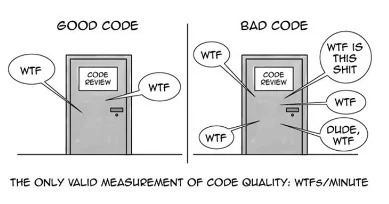
\includegraphics{wtf-per-minute}}\\
        Find guiding design principles to maintain software quality over time.
      \end{center}
    \end{minipage}
  \end{center}
\end{slide}

\begin{slide}
  \pdfbookmark[1]{Software Rot}{software-rot}
  \heading{Software Rot}
  \begin{center}
    \textbf{Symptoms of rotting software design:}\footnote{Robert C. Martin: Design Principles and Design Patterns}
    \begin{itemize}
      \item \textbf{Rigidity}: software difficult (a lot of work) to change
      \item \textbf{Fragility}: changes easily break the software
      \item \textbf{Immobility}: it is easier to rewrite than reuse parts
      \item \textbf{Viscosity}: design preserving methods are harder to employ than hacks
    \end{itemize}
  \end{center}
\end{slide}

\begin{slide}
  \pdfbookmark[1]{Aims}{aims}
  \heading{Aims}
  \begin{center}
    \textbf{In contrast we want to achieve the following:}\footnote{Robert C. Martin: Design Principles and Design Patterns}\medskip\\
    \begin{minipage}[c]{.65\textwidth}
      \begin{itemize}
        \item Keep software application \textbf{flexible}
        \item Keep software application \textbf{robust}
        \item Keep software application \textbf{reusable}
        \item Keep software application \textbf{developable}
      \end{itemize}
    \end{minipage}
  \end{center}
\end{slide}

\begin{slide}
  \pdfbookmark[1]{Robert C. Martin, Michael Feathers}{martin-feathers}
  \heading{Robert C. Martin, Michael Feathers}
  \begin{center}
    \begin{minipage}[b]{.25\textwidth}
      \begin{center}
        \resizebox*{.93\textwidth}{!}{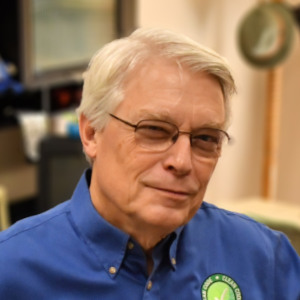
\includegraphics{robert-martin}}\\
        Robert C. Martin\bigskip\\
      \end{center}
    \end{minipage}
    \begin{minipage}[b]{.7\textwidth}
      \begin{itemize}
        \item One of \href{https://agilemanifesto.org/}{Agile Manifesto}'s authors
        \item Author of \href{https://www.informit.com/store/clean-code-a-handbook-of-agile-software-craftsmanship-9780132350884}{Clean Code}, \href{https://www.informit.com/store/functional-design-principles-patterns-and-practices-9780138176396}{Functional Design}, and more books
        \item Author of \href{https://web.archive.org/web/20150906155800/http://www.objectmentor.com/resources/articles/Principles_and_Patterns.pdf}{Design Principles and Design Patterns} paper based on his experience working at Xerox and other companies
      \end{itemize}
    \end{minipage}\\\rule{.95\textwidth}{1pt}
    \begin{minipage}[b]{.25\textwidth}
      \begin{center}
        \resizebox*{.93\textwidth}{!}{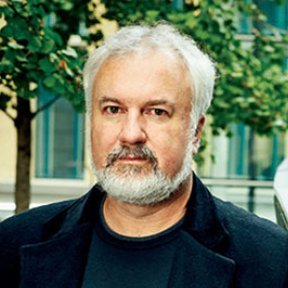
\includegraphics{michael-feathers}}\\
        Michael Feathers
      \end{center}
    \end{minipage}
    \begin{minipage}[b]{.7\textwidth}
      \begin{itemize}
        \item Author of \href{https://www.informit.com/store/working-effectively-with-legacy-code-9780131177055}{Working Effectively With Legacy Code}
        \item Summarized Robert C. Martin's paper using the SOLID acronym
      \end{itemize}
    \end{minipage}
  \end{center}
\end{slide}

\begin{slide}
  \pdfbookmark[1]{The SOLID Principles}{solid-principles}
  \heading{The SOLID Principles}
  \begin{center}
    \begin{Large}
      \begin{minipage}[c]{.6\textwidth}
        \begin{enumerate}
          \item \textbf{S}ingle responsibility
          \item \textbf{O}pen-closed
          \item \textbf{L}iskov substitution
          \item \textbf{I}nterface segregation
          \item \textbf{D}ependency inversion
        \end{enumerate}
      \end{minipage}
    \end{Large}
  \end{center}
\end{slide}

\begin{slide}
  \pdfbookmark[1]{Single Responsibility}{single-responsibility}
  \pdfbookmark[2]{Before}{single-responsibility-before}
  \heading{Single Responsibility - Before}
  \begin{center}
    \begin{minted}{python}
def adults_to_html(people):
    result = "<ul>\n"
    for person in people:
        if person.age >= 18:
            result += "  <li>" + person.name + "</li>\n"
    result += "</ul>"
    return result
# ...
page = adults_to_html(people)
    \end{minted}
  \end{center}
\end{slide}

\begin{slide}
  \pdfbookmark[2]{After}{single-responsibility-after}
  \heading{Single Responsibility - After}
  \begin{center}
    \begin{minted}{python}
def select_adults(people):
    return [person for person in people if person.age >= 18]

def people_to_html(people):
    result = "<ul>\n"
    for person in people:
        result += "  <li>" + person.name + "</li>\n"
    result += "</ul>"
    return result
# ...
page = people_to_html(select_adults(people))
    \end{minted}
  \end{center}
\end{slide}

\begin{slide}
  \pdfbookmark[1]{Open-Closed}{open-closed}
  \pdfbookmark[2]{Before}{open-closed-before}
  \heading{Open-Closed - Before}
  \begin{center}
    \begin{minted}{python}
def total_area(shapes):
  result = 0
  for shape in shapes:
    match type(shape):
      case Rectangle:
        result += shape.width * shape.height
      case Sphere:
        result += math.pi * shape.radius ** 2
      case _:
        raise f"Unsupported shape {shape}"
  return result
    \end{minted}
  \end{center}
\end{slide}

\begin{slide}
  \pdfbookmark[2]{After}{open-closed-after}
  \heading{Open-Closed - After}
  \begin{center}
    \begin{minted}{python}
class Rectangle:
  def area(self):
    return self.width * self.height

class Circle:
  def area(self):
    return math.pi * self.radius ** 2

def total_area(shapes):
  result = 0
  for shape in shapes:
    result += shape.area()
  return result
    \end{minted}
  \end{center}
\end{slide}

\begin{slide}
  \pdfbookmark[1]{Liskov-Substitution}{liskov-substitution}
  \pdfbookmark[2]{Before}{liskov-substitution-before}
  \heading{Liskov-Substitution - Before}
  \begin{center}
    \begin{minted}{python}
class Rectangle:
  def __init__(self, width, height):
    self.width = width
    self.height = height
  def set_width(self, width):
    self.width = width
  def set_height(self, height):
    self.height = height

class Square(Rectangle):
  def __init__(self, side):
    super().__init__(side, side)
  def set_width(self, width):
    super().set_width(width)
    super().set_height(width)
  def set_height(self, height):
    self.set_width(height)
    \end{minted}
  \end{center}
\end{slide}

\begin{slide}
  \pdfbookmark[2]{After}{liskov-substitution-after}
  \heading{Liskov-Substitution - After}
  \begin{center}
    \begin{minipage}[c]{.6\textwidth}
      \begin{minted}{python}
class Shape:
  pass

class Rectangle(Shape):
  def __init__(self, width, height):
    self.width = width
    self.height = height
  def set_width(self, width):
    self.width = width
  def set_height(self, height):
    self.height = height

class Square(Shape):
  def __init__(self, side):
    self.side = side
  def set_side(self, side):
    self.side = side
      \end{minted}
    \end{minipage}
    \begin{minipage}[c]{.35\textwidth}
      \begin{center}
        \resizebox*{.93\textwidth}{!}{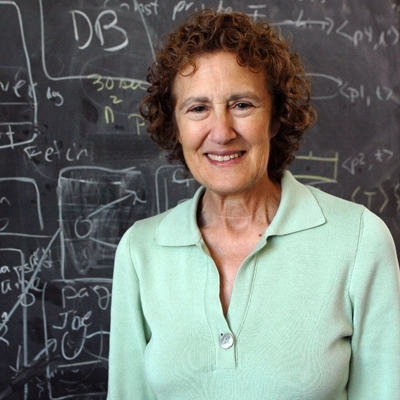
\includegraphics{barbara-liskov}}\\
        Barbara Liskov
      \end{center}
    \end{minipage}
  \end{center}
\end{slide}

\begin{slide}
  \pdfbookmark[2]{Contracts}{liskov-substitution-contracts}
  \heading{Liskov-Substitution - Contracts}
  \begin{center}
    ``The Liskov Substitution Principle states, among other constraints, that a subtype is not substitutable for its super type
    if it strengthens its operations' preconditions, or weakens its operations' postconditions''\footnote{\href{https://www.cs.ubc.ca/~ebani/papers/LiskofHappySad_ICSE-SEET_2018.pdf}{Baniassad: Making the Liskov Substitution Principle Happy and Sad}}\bigskip\\
    \resizebox*{.8\textwidth}{!}{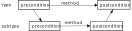
\includegraphics{liskov}}
  \end{center}
\end{slide}

\begin{slide}
  \pdfbookmark[1]{Interface Segregation}{interface-segregation}
  \pdfbookmark[2]{Before}{interface-segregation-before}
  \heading{Interface Segregation - Before}
  \begin{center}
    \begin{minted}{python}
class AccountHolder:
  def __init__(self, name, age, balance):
    self.name = name
    self.age = age
    self.balance = balance
  def is_adult(self):
    return self.adult >= 18
  def deposit(self, amount):
    self.balance += amount
  def withdraw(self, amount):
    self.balance -= amount
    \end{minted}
  \end{center}
\end{slide}

\begin{slide}
  \pdfbookmark[2]{After}{interface-segregation-after}
  \heading{Interface Segregation - After}
  \begin{center}
    \begin{minted}{python}
class Person:
  def __init__(self, name, age):
    self.name, self.age = name, age
  def is_adult(self):
    return self.adult >= 18

class Account:
  def __init__(self, balance):
    self.balance = balance
  def deposit(self, amount):
    self.balance += amount
  def withdraw(self, amount):
    self.balance -= amount

class AccountHolder(Person):
  def __init__(self, name, age, account):
    super().__init__(name, age)
    self.account = account
    \end{minted}
  \end{center}
\end{slide}

\begin{slide}
  \pdfbookmark[1]{Dependency Inversion}{dependency-inversion}
  \pdfbookmark[2]{Before}{dependency-inversion-before}
  \heading{Dependency Inversion - Before}
  \begin{center}
    \begin{minted}{python}
def get_names(connection):
    cursor = connection.cursor()
    cursor.execute('SELECT name FROM member_table')
    rows = cursor.fetchall()
    names = [row[0] for row in rows]
    return names

connection = sqlite3.connect('example.db')
names_list = get_names(connection)
connection.close()
print(names_list)
    \end{minted}
  \end{center}
\end{slide}

\begin{slide}
  \pdfbookmark[2]{After}{interface-segregation-after}
  \heading{Dependency Inversion - After}
  \begin{center}
    \begin{minted}{python}
class Database(abc.ABC):
  @abc.abstractmethod
  def sql(self, query):
    pass

class SQLiteDatabase(Database):
  def __init__(self, db_file_name):
    self.connection = sqlite3.connect(db_file_name)
  def __del__(self):
    self.connection.close()
  def sql(self, query):
    cursor = self.connection.cursor()
    cursor.execute(query)
    return cursor.fetchall()

def get_names(database):
  rows = database.sql('SELECT name FROM member_table')
  return [row[0] for row in rows]
    \end{minted}
  \end{center}
\end{slide}

\begin{slide}
  \heading{Dependency Inversion - After}
  \begin{center}
    \begin{minted}{python}
database = SQLiteDatabase('example.db')
names_list = get_names(database)
print(names_list)
    \end{minted}
  \end{center}
\end{slide}

\begin{slide}
  \pdfbookmark[1]{Aspects of a Class}{class-aspects}
  \heading{Aspects of a Class}
  \begin{center}
    \textbf{The 5 aspects of the class are:}\footnote{\href{https://swarch.blog/the-five-principles-for-solid-software-design/}{Mike Lindner: The Five Principles For SOLID Software Design}}\\
    \resizebox*{.6\textwidth}{!}{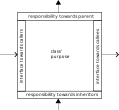
\includegraphics{aspects}}
  \end{center}
\end{slide}

\begin{slide}
  \pdfbookmark[1]{Principles of a Class}{class-aspects}
  \heading{The 5 Principles}
  \begin{center}
    \textbf{The 5 corresponding principles are:}\footnote{\href{https://swarch.blog/the-five-principles-for-solid-software-design/}{Mike Lindner: The Five Principles For SOLID Software Design}}\\
    \resizebox*{.6\textwidth}{!}{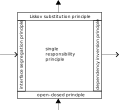
\includegraphics{principles}}
  \end{center}
\end{slide}

\begin{slide}
  \pdfbookmark[1]{Arjan Egges on SOLID}{arjancodes-video}
  \heading{Arjan Egges: Uncle Bob's SOLID Principles Made Easy}
  \begin{center}
    \href{https://www.youtube.com/watch?v=pTB30aXS77U}{\resizebox*{.95\textwidth}{!}{
\includegraphics{arjancodes}}}\\
    {\small 19 minutes video}
  \end{center}
\end{slide}

\begin{slide}
  \pdfbookmark[1]{Jim Weirich on Connascence}{weirich-video}
  \heading{Jim Weirich: The Building Blocks of Modularity}
  \begin{center}
    \href{https://www.youtube.com/watch?v=q85rdBMe9GY}{\resizebox*{.95\textwidth}{!}{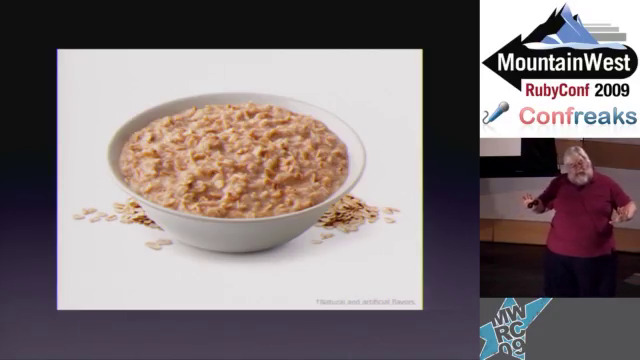
\includegraphics{weirich}}}\\
    {\small 33 minutes video}
  \end{center}
\end{slide}

\end{document}
